%\addcontentsline{toc}{chapter}{Kapitel-1}
\chapter{Partikel Erkennung}

In diesem  Abschnitt werden einige Möglichkeiten zur Erkennung von Partikeln in einem Video niedriger Auflösungsqualität verglichen und hervorgehoben. Es wäre natürlich ideal einen Vergleich zwischen manuellen und werkzeugbasierten Erkennung zu ziehen. Aber leider wird die manuelle Erkennung hier nicht vollzogen aufgrund der viel zu schwierig bzw. langwierige Arbeit, die es bereitet. Es geht hier nämlich um mehrere hunderte von Partikeln pro Bild. 
\todo{ ToDo: Ein Bild soll hier als Beispiel verwiesen werden.}
\\

In diesem Sinne widmet sich die Arbeit in der Folgezeit dem Vergleich möglicher Werkzeugen, die zur Erreichung der eigentlichen Ziele nutzen können. Hierbei werden aus der Vielzahl der Instrumente nur vier oder fünf herausgegriffen. Diese werden zunächst einer tabellarischen Grobanalyse der Merkmale und dann einer textuellen Analyse der Unterschiede unter ihnen unterzogen. \\

\todo{ ToDo: Zwei weitere Partikel-Tracking-Bibliotheken finden.}
\todo{ ToDo: Eigenschaften jeglicher Tool im Vergleich Anderer zu herausfinden}

\begin{tabular}{|c||c|c|l|}
\hline
Werkzeug & Schwerpunkt & Zugänglichkeit & Parameteranzahl \\
\hline
\hline
 TrackPy & & & \\
 \hline
 PyPIV   & & & \\
 \hline
 OpenPTV & & & \\
 \hline
 STracking  & & & \\
 \hline
 PySTACHIO  & & & \\
 \hline
\end{tabular}

\todo{\href{file:///C:/Users/leb/Downloads/10.21105.joss.04398.pdf}{MyPTV}, \\ \href{https://www.sciencedirect.com/science/article/pii/S2001037021002944}{PySTACHIO},\\ \href{https://spt.readthedocs.io/en/latest/}{SPT}
\\ \href{https://www.google.com/search?q=Python+package+for+particle+tracking&rlz=1C1CHBF_deDE987DE987&sxsrf=ALiCzsYl2NtGnlFYYupES17uNyNLp8zhIQ:1653590912505&ei=gMuPYoKwHsyMxc8Phquk2AM&start=10&sa=N&ved=2ahUKEwiC8MWX6v33AhVMRvEDHYYVCTsQ8NMDegQIARBQ&biw=1920&bih=969}{Python package for particle tracking}}


%\addcontentsline{toc}{section}{Kapitel-1}
\section{Werkzeugbasierte Erkennung}

\subsection{Trackpy}
Trackpy ist ein Python-Paket, das es ermöglicht aus einem Video bzw. einer Imagesequenz Partikel in unterschiedlichen Dimensionen (2D und 3D) zu erkennen und zu verfolgen. Hier wird es natürlich die Zweidimensionalität anvisiert. Die Erkennung der Partikel erfolgt über eine der Funktionen des Paketes, nämlich die \textit{locate-}Funktion.
Dieser verfügt über eine reihe von Parametern, anhand derer die Qualität der Anerkennung ausgebessert werden kann.

	\subsubsection{Parameter der locate-Funktion}
		Folgende Parameter werden im Laufe dieser Arbeit angewandt:

		\begin{enumerate}
    			\item raw\_image: array \\
    			Wird für die endgültige Charakterisierung verwendet.
    			\item diameter: odd integer \\
    			Entspricht der geschätzten Größe der Partikeln (in Pixel).
    			\item minmass: float \\
    			Minimale eingebaute Helligkeit. Dies ist ein Schlüsselparameter, um störende 				Merkmale zu entfernen. Der Standardwert ist es 'None'.
%    			\item maxsize: float\\
%    			Maximaler Gyrationsradius der Helligkeit.
    			\item separation: float\\
    			Minimaler Abstand zwischen den Partikeln. Der Standardwert ist \textit{diameter + 1}   			
    			\item noise\_size: float or tuple\\
    			Breite des Gaußschen Unschärfekerns, in Pixeln. Der Standardwert ist 1.
    			\item topn: interger\\
    			Gibt lediglich die N hellsten Merkmale über minmass zurück. Wenn 							'None' (Voreinstellung), werden sämtliche Eigenschaften oberhalb von minmass 				zurückgegeben.
%    			\item preprocess: boolean\\
%    			Vorverarbeitung der Bandpass .
    			\item max\_iterations: interger\\
    			Maximale Anzahl der Schleifen zur Verfeinerung des Massenschwerpunkts, 					Standardwert 10.
%    			\item filter\_after: boolean\\
    			
		\end{enumerate}
		
Ein \textsc{Panda.Dataframe} mit den Daten \textit{y\-koordinaten, x\-koordinaten, mass, size, ecc, signal, raw\_mass, ep, frame} wird als Rückgabewert geworfen. Dies gilt für jedes der gefundenen Partikel.(Siehe )
Ausführlichere Informationen zu  weiteren Parametern sowie zu den Obengennanten ist auf zu ist.%~ \citep{Tp}% zu sehen. 
An dieser Stelle kann folgende Frage aufgeworfen werden: Was sind die besten Parameter? \\
Beachte, dass einfachheitshalber, während der gesamten Parametereinstellung nur das erste Bild unseres Videos betrachtet wird.

	\subsubsection{Welche sind die optimalen Parameterwerte für eine ideale Partikelerkennung?}
	Hier wird es ein Antwortversuch auf die zuletzt gestellte Frage eingegangen. Zur Erreichung dieses Zieles wird mit der Erkennung begonnen, indem nur die geforderten Parameter(raw\_image und diameter) verwendet werden und nach und nach weitere hinzugefügt werden, um die Suche zu verfeinern. 
	
	\begin{enumerate}
    			\item \textbf{locate(f, d): Wobei f = raw\_image und d = diameter.} \\ \\
    			 Während frames[0] entspricht in diesem Fall dem ersten Bild der Videoaufnahme bzw. der Imagesequenz. \texttt{frames} hingegen bilden die Gesamtheit der Bilder des Videos im Laufe der Zeit und damit die Sequenz der Bilder.  Diese Angabe, die vom Typ Array ist, stellt eine Voraussetzung für die Ausführung von Funktionen dar. \\
    			 Für den Durchmesser wird zunächst willkürlich eine ziemlich kleine ungerade Zahl genommen, um die Ergebnisse zu sehen und eine Annäherung an den Wert, den wir verwenden sollen, zu erhalten. Zunächst nehmen wir also einen Durchmesser von drei (d=3).  
    			 
\begin{figure}[H]
    \centering
    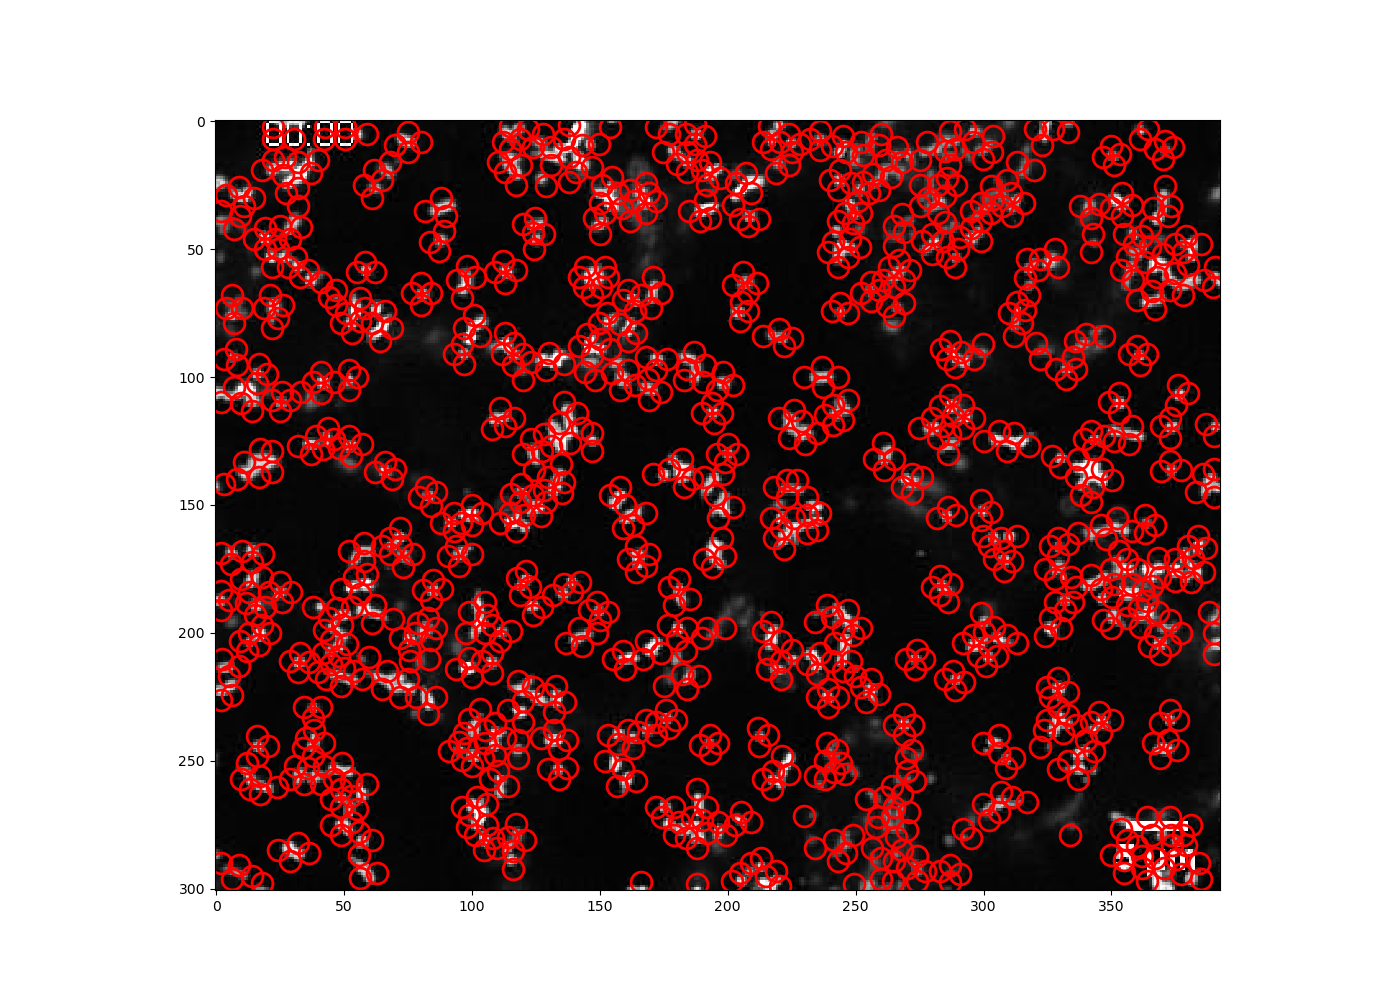
\includegraphics[scale=0.35]{Grafiken/trackpyBilder/locate(f0, diameter=3).png}
    \caption{locate(frames[0], 3)}
    \label{fig:bild_label}
\end{figure} 

Das Bild zeigt eine potente Lokalisierung der Partikel. Es wurde dabei fast alle Elemente des Bildes erkannt, wobei offensichtlich eine deutlich große Menge \textit{false Positive} ist. \\
Eine Verfeinerung der Lokalisierung würde somit einen größeren Durchmesser erfordern. Dies erfolgt in der Folge durch die Verwendung einer immer noch ungeraden Zahl, die jedoch einen größeren Wert hat. In diesem Fall ist es neun, da es so viele "False Positives" gibt. 
\texttt{locate(frames[0], 9)}

\begin{figure}[H]
    \centering
    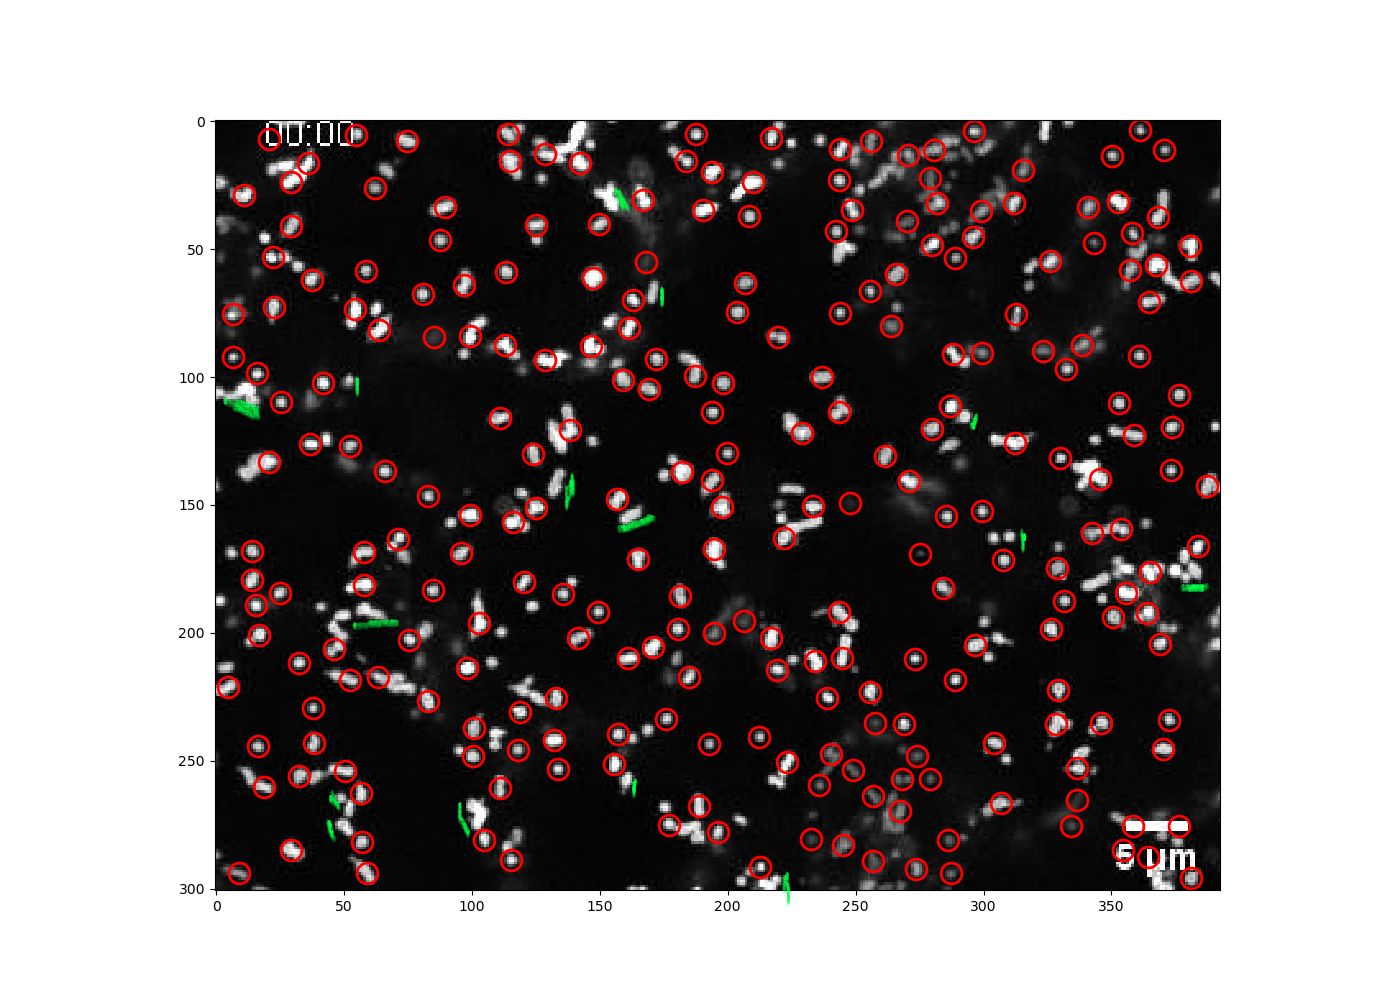
\includegraphics[scale=0.35]{Grafiken/trackpyBilder/locate(frames[0], 9).png}
    \caption{locate(frames[0], 9)}
    \label{fig:bild_label}
\end{figure} 

Diesmal gibt es zwar viel weniger ungewollte Teilchen. Allerdings hat sich eine große Anzahl von "False Negatives" gebildet. \\
Aus diesem Grund wurde nacheinander der Durchmesser von sieben und dann von fünf ausprobiert.\\
\texttt{locate(frames[0], 7)}   gefolgt  \texttt{locate(frames[0], 5)}
\newpage

\begin{figure}[H]
    \centering
    \begin{minipage}{.5\textwidth}
     	\centering
  	  	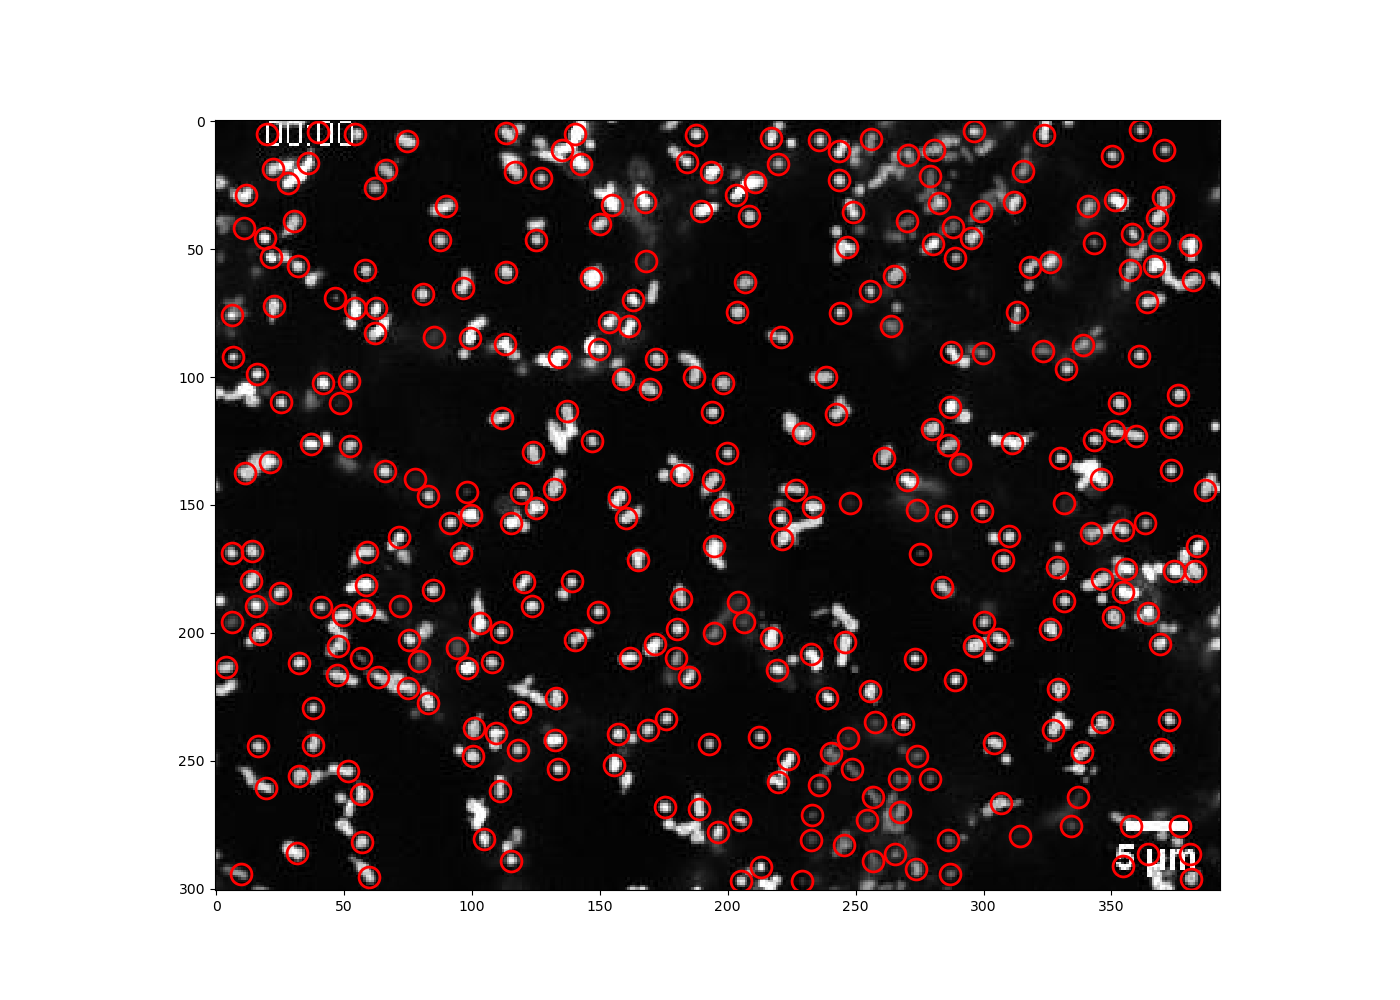
\includegraphics[scale=0.3]{Grafiken/trackpyBilder/locate(frames[0], 7).png}
 	 	\captionof{figure}{locate(frames[0], 7)}
 		\label{fig:test1}
    \end{minipage}
	
	\begin{minipage}{.5\textwidth}
     	\centering
  	  	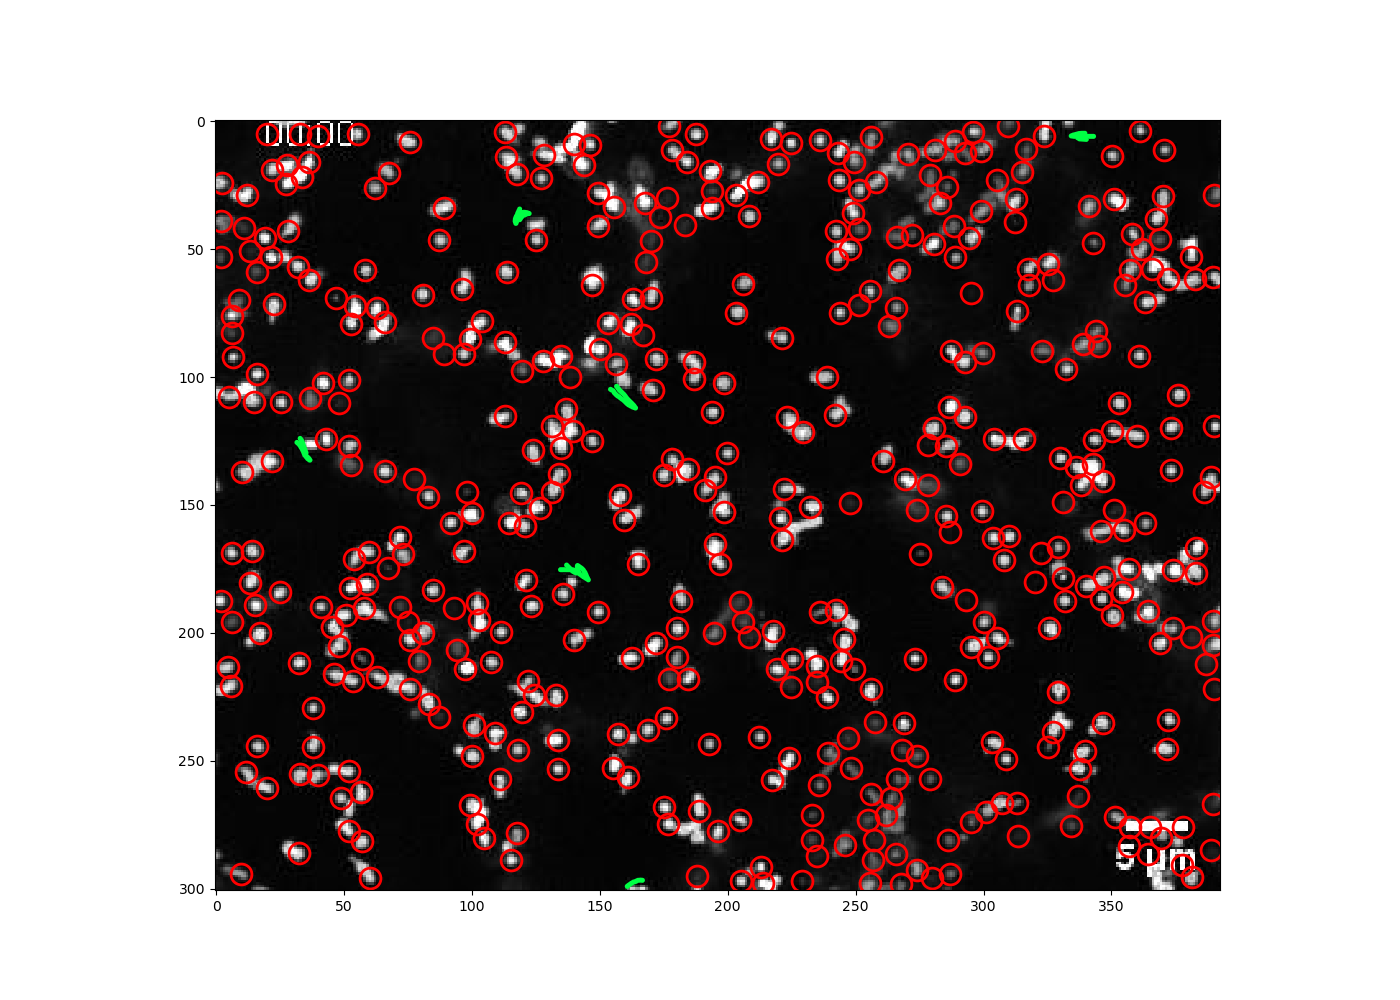
\includegraphics[scale=0.3]{Grafiken/trackpyBilder/locate(frames[0], 5).png}
 	 	\captionof{figure}{locate(frames[0],5)}
 		 \label{fig:test2}
    \end{minipage}
\end{figure}

In Anbetracht des Ziels, einen Durchmesser zu finden, der die Erkennung möglichst vieler Partikel ermöglicht und gleichzeitig möglichst wenig unerwünschte Partikel enthält, ist es besser, mit dem Durchmesser 5 fortzufahren. Denn aus den zuvor verwendeten Durchmessern geht hervor, dass bei diesem Bild die Anzahl der nicht-lokalisierten Teilchen umso größer ist, je höher der Durchmesser ist. 
Dies ist nicht als Allgemeingültigkeit zu verstehen, da verschiedene Videos unterschiedliche Arten von Partikeln mit variierenden Größen und Dicken aufweisen. Es wäre ratsam, die Parameter bei jedem neuen Video zu testen.
Tatsächlich lassen sich insgesamt 475 Partikeln finden, von denen ca. 121 unerwünscht waren und kaum fehlten. Dies entspricht einer ungefähren Rate von 25.47\%.

\begin{figure}[H]
    \centering
    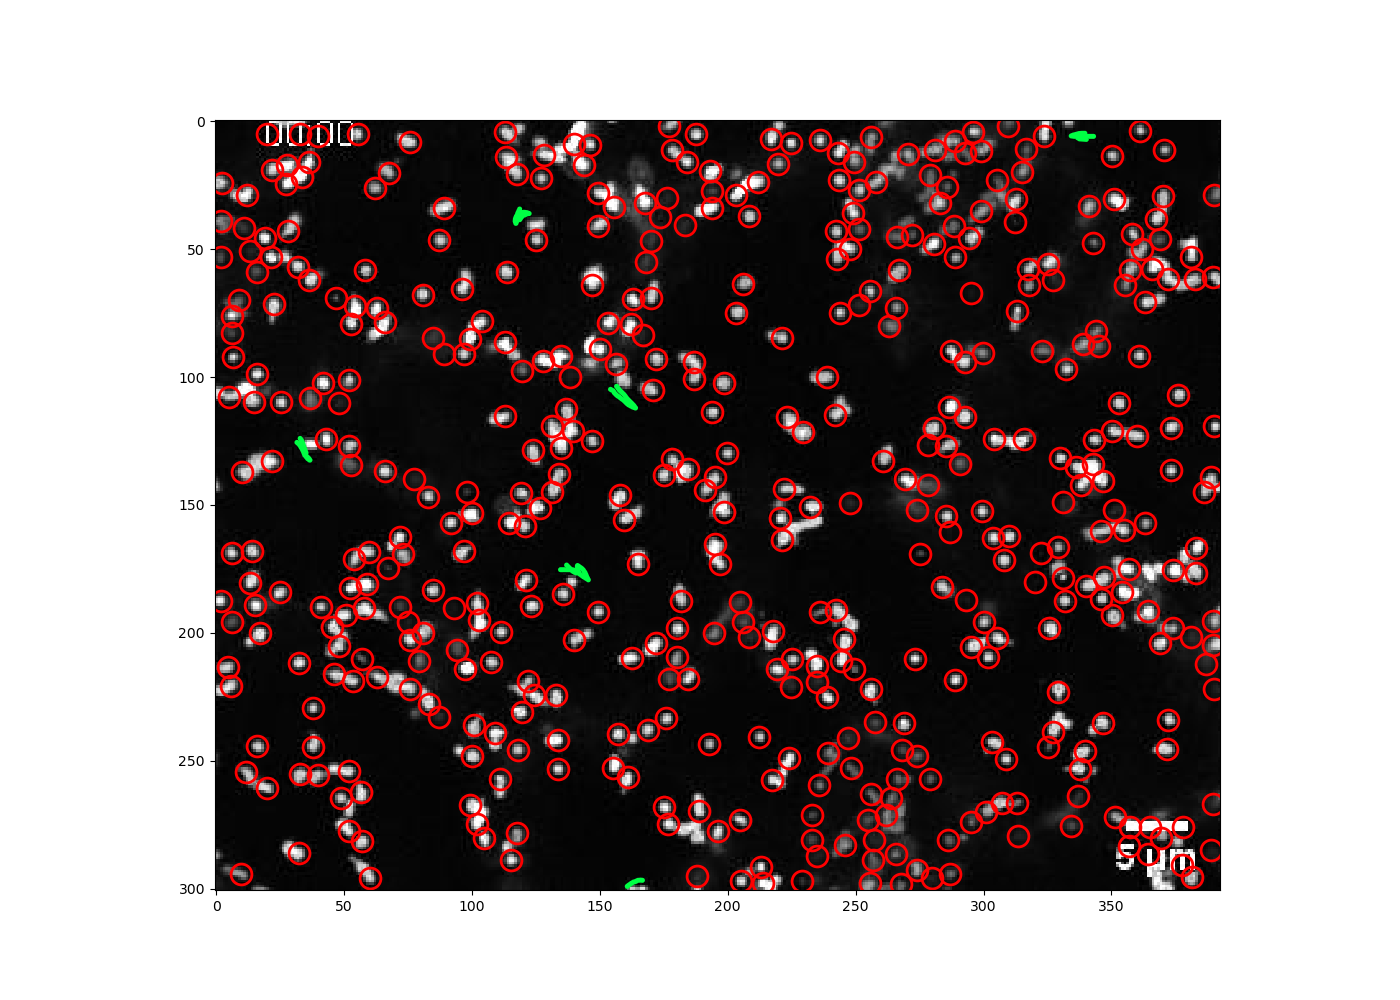
\includegraphics[scale=0.35]{Grafiken/trackpyBilder/locate(frames[0], 5).png}
    \caption{locate(frames[0], 5)}
    \label{fig:bild_label}
\end{figure} 
%    			 In diesem Sinne sieht das Ergebnis der Lokalisierung ohne weitere Parameter wie folgt aus:
%\begin{figure}[H]
%    \centering
%    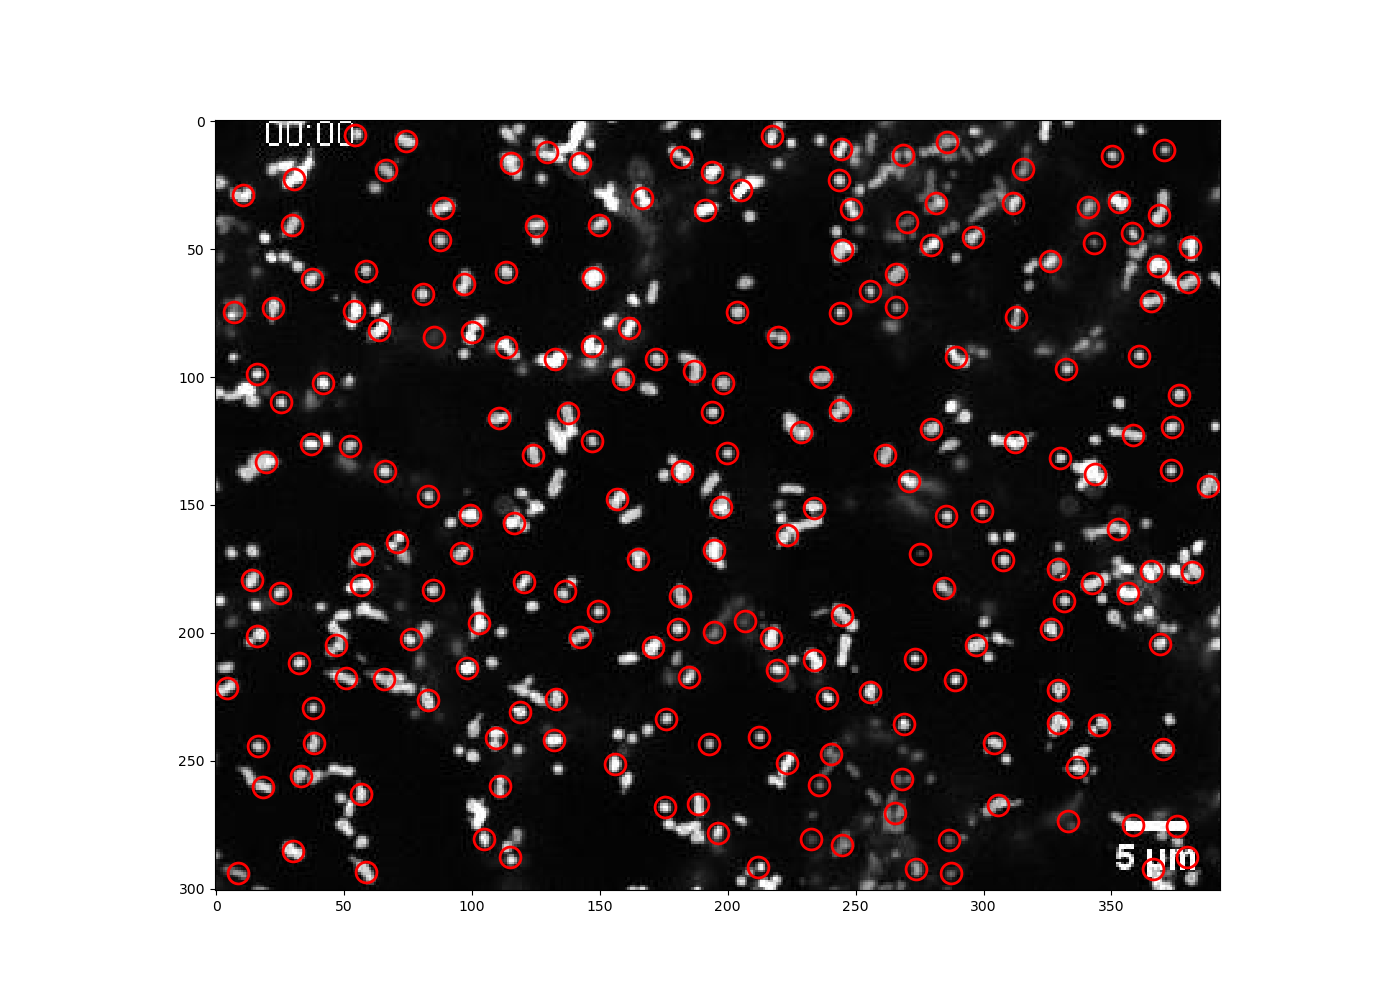
\includegraphics[scale=0.35]{Grafiken/trackpyBilder/locate_with_required_parameter.png}
%    \caption{locate with needed Parameters}
%    \label{fig:bild_label}
%\end{figure}
%    			Wie auf dem \ref{fig:bild_label} zu sehen ist, wurde eine Menge an Partikel 
%    			nicht erkannt, während andere unerwünschten erkannt wurden. 
%    			Insgesamt lassen sich 207 Partikeln finden, von denen 22 unerwünscht waren  und 91 fehlten. Dies entspricht einer ungefähren Rate von 10,628\% für die unerwünschten und einer Rate von 43,9617\% für die nicht gefundenen.

    			
    			\item {\Large \textbf{locate(f, d, minmass)}}:\\ \\
%    			Da ca. nur 10\% der letzten Suche unerwünschte Elemente waren, wird den Durchschnitt der \textit{minmass} aller Teilchen berechnet und als \textit{minmass} verwendet. Aus der vorherigen \textsc{Panda.Dataframe} genügt es den Mittelwert aus den Werten der \textit{mass}-Spalte zu berechnen, um auf \textit{minmass} von ca. 2490.21 zu gelangen. Das Resultat wird dann wie folgt aussehen:
Wie bereits erwähnt, spiegelt \textit{minmass} die inhärente und eingebaute minimale Helligkeit jedes lokalisierten Partikels wider. Das Ziel ist es nun, die zuvor ermittelten, zu dunklen Partikel herauszufiltern. Daher ist es notwendig, methodisch mit dem Parameter \textit{minmass} zu spielen, um dieses Ziel zu erreichen. Es gibt natürlich mehrere Möglichkeiten, den optimalen Wert für die gesuchte Parameter zu finden. Allerdings wird hier die folgende Logik verfolgt:\\

Aus dem DataFrame der letzten Suche (locate(frames[0], 5)) wurde ja 475 Partikel gefunden. Davon sind ca. 25.47\%, also 121 unerwünscht. Diese Zahl entspricht so fast allen gefundenen zu dunklen Partikel. In anderen Worten, stellt sie die Elemente dar, deren \textit{minmass} zu niedrig ist.
So könnte der Dataframe verwendet werden und ihn nach der Spalte \textit{mass} absteigend sortieren. 
Dies würde dazu führen, dass unsere dunkelsten Partikel am Ende der Liste (Tabelle) positioniert werden und die hellsten ganz oben. Dazu muss keine Funktion implementiert werden, sondern es genügt, die Funktion \textit{sort\_values()} aus der Panda. Dataframe-Bibliothek aufzurufen. Der Aufruf sowie die Tabelle sähe jeweils dann wie folgt aus:\\ \texttt{dataframe.sort\_values(by=['mass'], ascending=False)}

\begin{figure}[H]
    \centering
    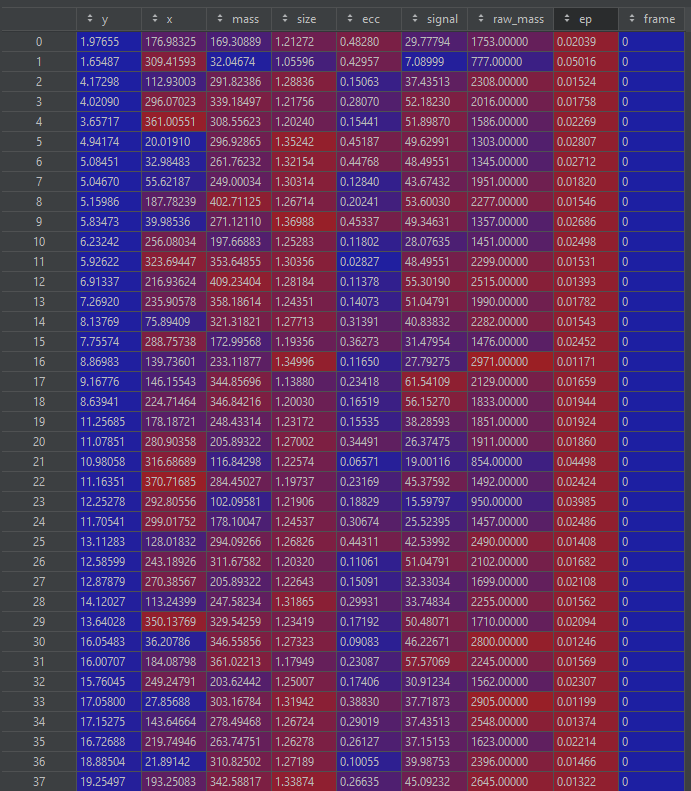
\includegraphics[scale=0.45]{Grafiken/trackpyBilder/df_initial.png}
    \caption{Ein Teil des initialen Dataframes}
    %\label{fig:bild_label}
\end{figure}

\begin{figure}[H]
    \centering
    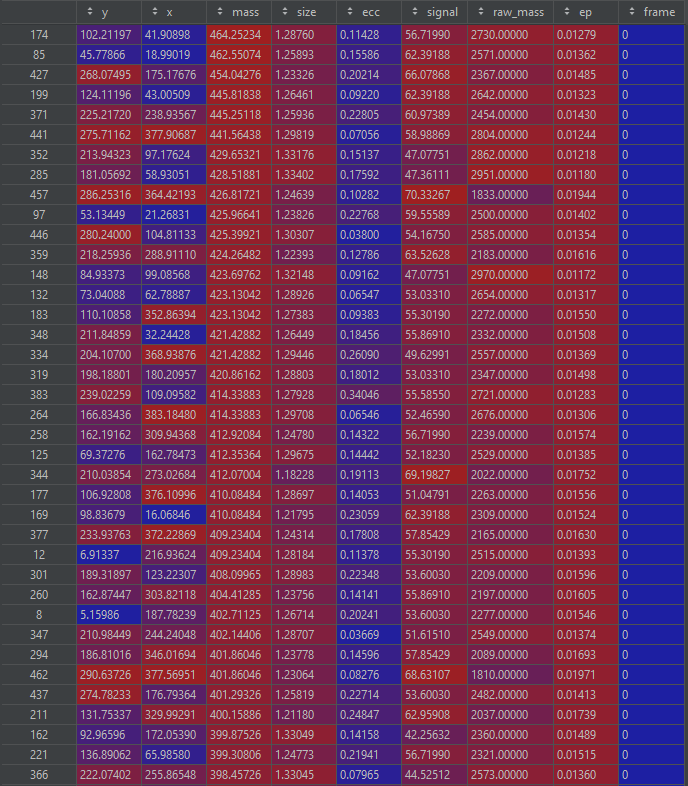
\includegraphics[scale=0.45]{Grafiken/trackpyBilder/df_sorted.png}
    \caption{Ein Teil des sortierten Dataframes}
    %\label{fig:bild_label}
\end{figure}

Jetzt wird es auf dem sortierten Dataframe eine weitere Funktion aufgerufen, um lediglich nur die 354 (also 475-121)gewünschte Partikel bwz. hellsten zu behalten. Eine solche Funktion \textit{head()} wird auch von Panda-Dataframe bereitgestellt. Aus diesem Ergebnis reicht es aus, die von Python angebotene Funktion \textit{min()} auszuführen, um den kleinsten Wert in der Spalte \textit{mass} zu erhalten. 
Die Aufrufe sähen dann wie folgt aus:\\
\texttt{dataframe.head(354)} \\
\texttt{min(dataframe['mass'])}\\

\textbf{189.72805} ist hier das Ergebnis der vorherigen Vorgänge und damit auch den minimalen Wert von \textit{mass}, den ein Partikel haben muss. Es sei der \textit{minmass} Parameter der Funktion \textit{locate()}.



%Es wurde zwar fast alle \textit{False Positive} beseitigt, aber dafür wurde eine viel zu hohe Anzahl an \textit{True Negative} nicht gefunden. Die Lösung für dieses Problem besteht darin, den Wert von "minmass"  schrittweise zu verringern, bis ein zufriedenstellendes Ergebnis erzielt wird.
\begin{figure}[H]
    \centering
    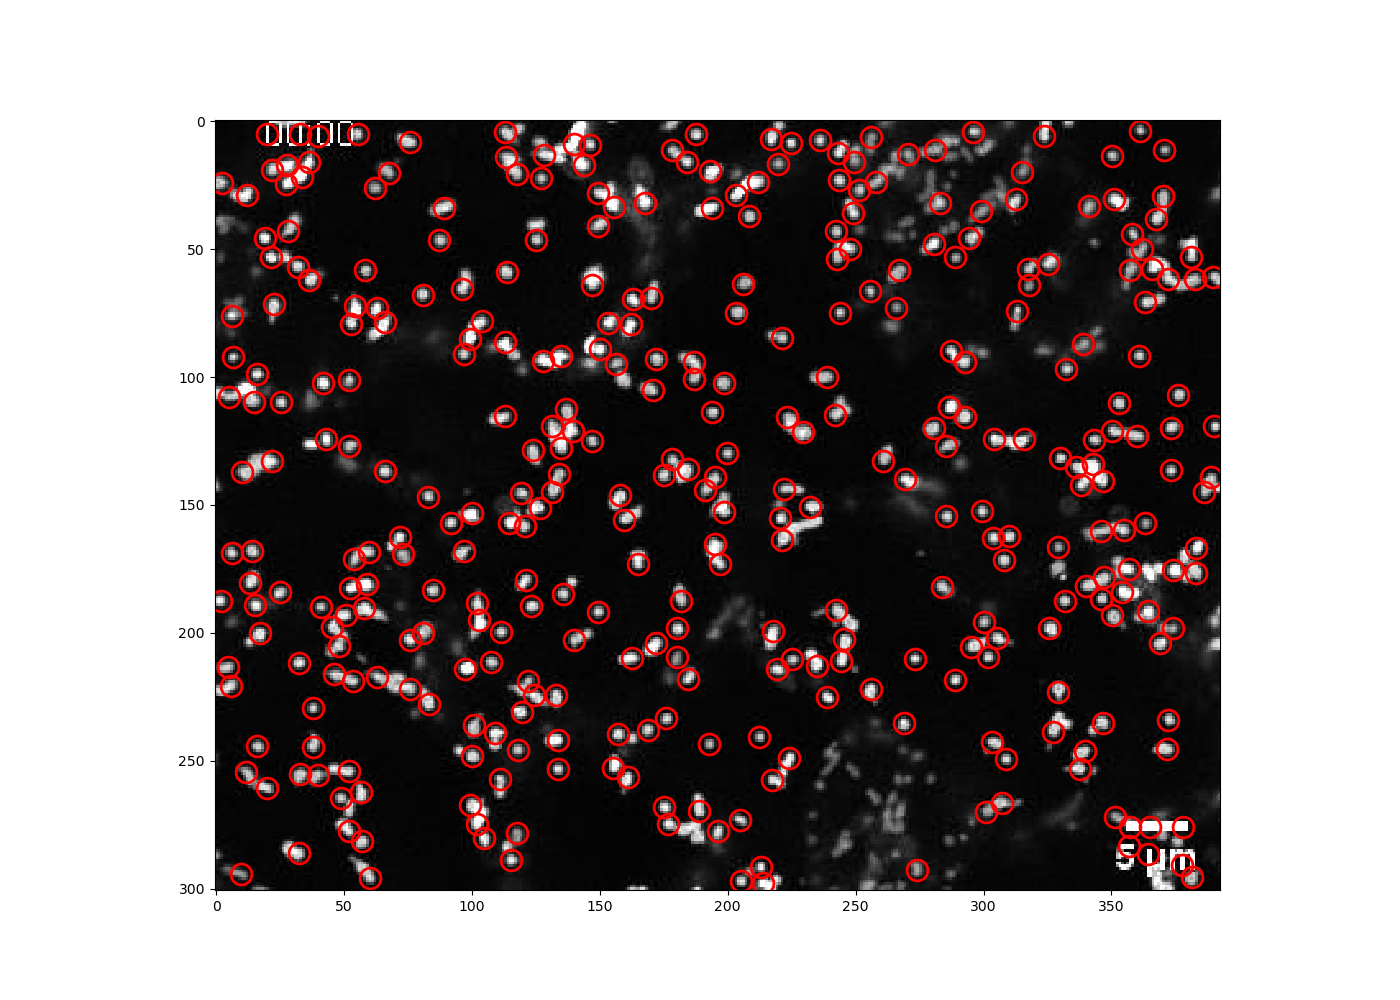
\includegraphics[scale=0.35]{Grafiken/trackpyBilder/locate_with_minmass_01.png}
    \caption{locate with 'mimass=189.72805'}
    %\label{fig:bild_label}
\end{figure}

Aus diesem Bild geht hervor, dass fast alle gewünschten Partikel lokalisiert bleiben. Allerdings werden einige von ihnen doppelt gezählt, was Gegenstand der Verwendung anderer Parameter sein wird. Dennoch gibt es noch einige Partikel, die nicht lokalisiert werden sollten. Es handelt sich dabei um etwa 12 Teilchen. Es wäre daher ratsam, die \textit{minmass} schrittweise zu erhöhen, bis ein zufriedenstellendes Ergebnis erzielt wird.\\
Zum Festlegen des Wertes, der in jedem Schritt verwendet werden soll, schauen Sie in der Tabelle (Dataframe), die mit \textit{dataframe.sort\_vaules(by=['mass'], ascending=False}) erstellt wurde, beginnend mit der 121. Zeile von unten nach oben.(121. Zeile entspricht der Anzahl der Teilchen mit geringer Helligkeit)

\begin{figure}[H]
    \centering
    \includegraphics[scale=0.55]{Grafiken/trackpyBilder/df\_steps.png}
    \caption{Sortierte Tabelle}
    %\label{fig:bild_label}
\end{figure}

So werden nach und nach die Werte 197,1016 (d. h. 197), 197,6688 (d. h. 198) und so weiter verwendet.\\
Die Verwendung der Funktion \texttt{locate(frames[0], 5, \textbf{minmass=197})} ergibt so gut wie keine Änderung der Lokalisierung. Da insgesamt immer noch 353 Partikel  erkannt wurde. Daher wird sich der nächste Versuch mit dem folgenden Wert beschäftigen. Genauer gesagt "minmass = 198". \\
Auch hier wurden nur zwei Teilchen weniger gefunden. Das sind insgesamt 351 Partikel. Obwohl es fast unmöglich ist, diese beiden Teilchen auf dem Bild zu erkennen. 
Es wäre klug, den nächsten Wert unserer Tabelle zu nehmen, der derzeit bei 203,6244 (also 204) liegt, und erneut zu versuchen, eine Lokalisierung durchzuführen. (Siehe )

\begin{figure}[H]
    \centering
    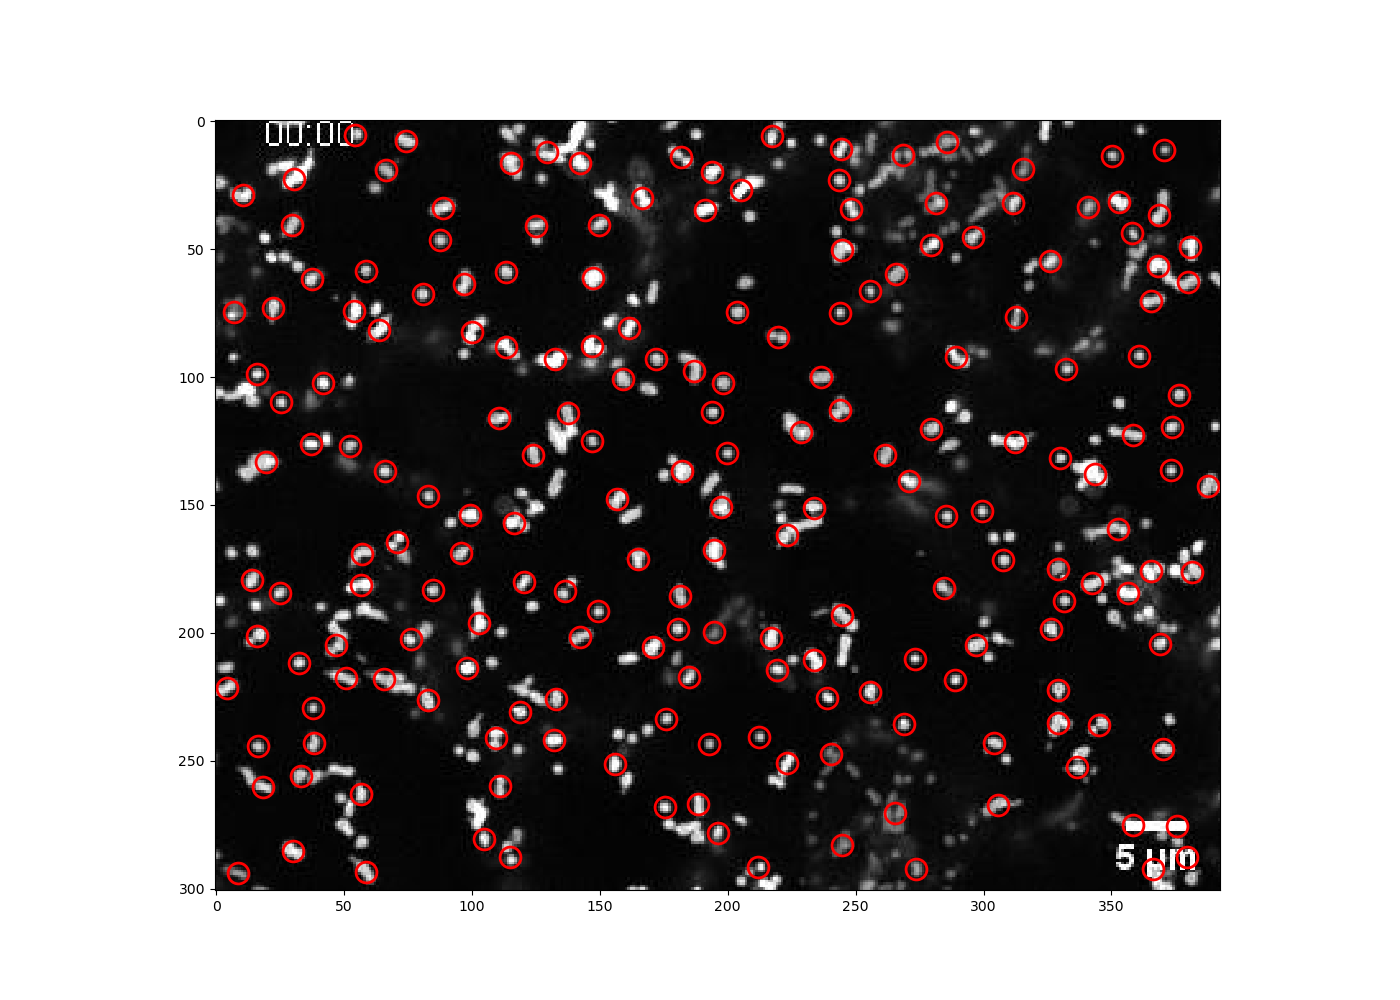
\includegraphics[scale=0.35]{Grafiken/trackpyBilder/locate_with_minmass_02.png}
    \caption{locate with 'mimass=197'}
    %\label{fig:bild_label}
\end{figure}


\begin{figure}[H]
    \centering
    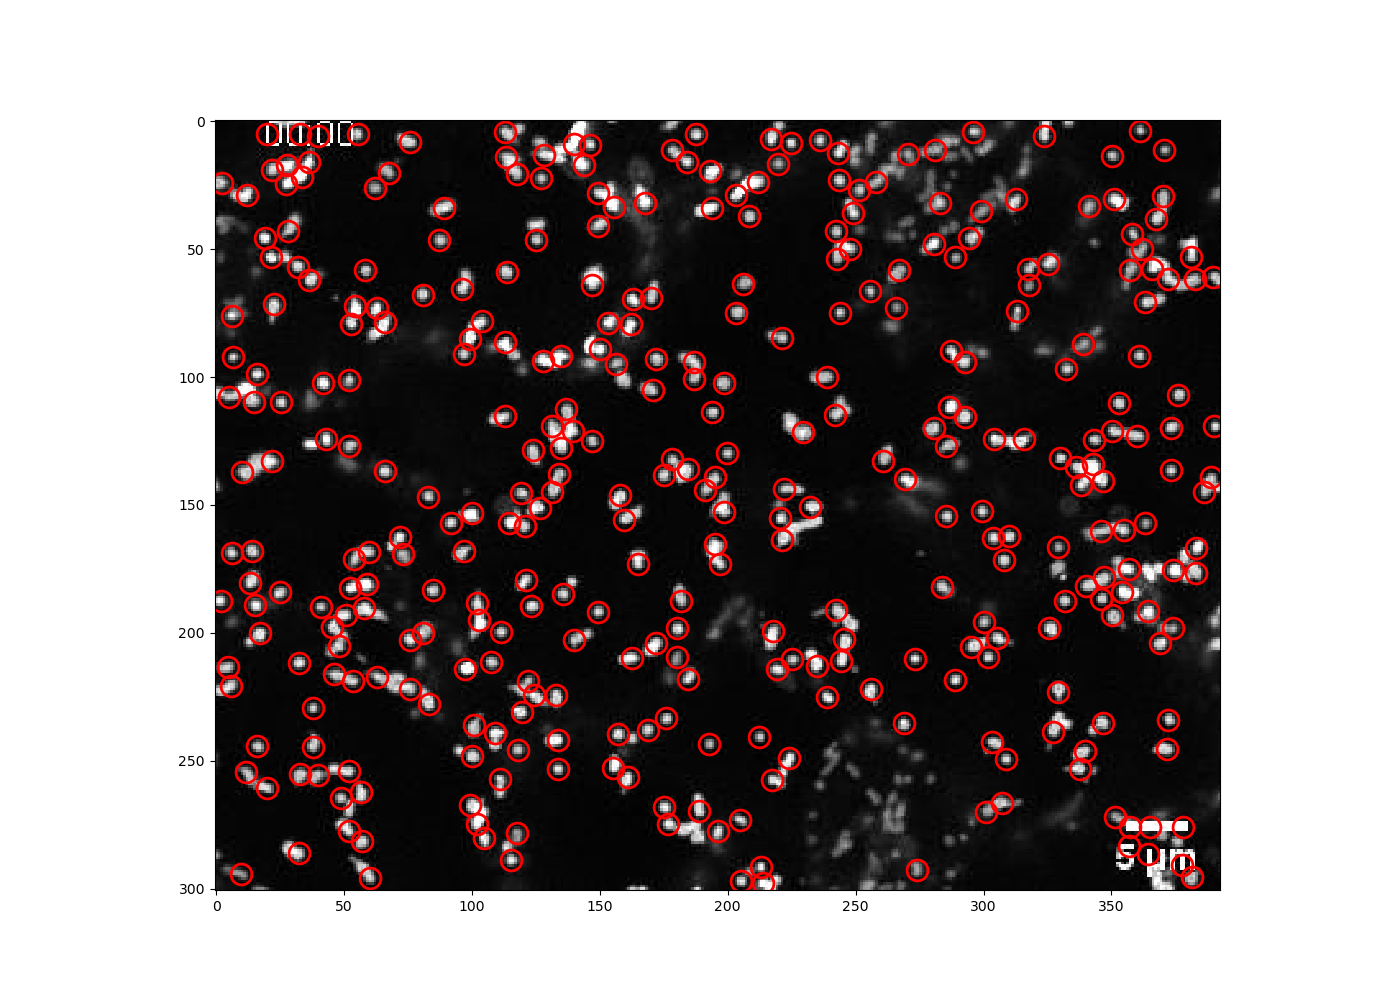
\includegraphics[scale=0.35]{Grafiken/trackpyBilder/locate_with_minmass_04(204).png}
    \caption{locate with 'mimass=204'}
    %\label{fig:bild_label}
\end{figure}

Bei der Verfolgung dieser Logik kommt es hier schnell auf einen \textit{minmass} Wert von \textbf{210}.\\
Wo es deutlich zu erkennen ist, dass weitere unerwünschte Partikel nicht mit erkannt wurde. Es wurde insgesamt hier \textbf{345} Partikel gefunden. Jedoch muss es festgestellt werden, dass ab \textbf{211} nach oben, werden zwar weniger unerwünschte Partikel gefangen, aber auch erwünschte. 
Wie es die Veranschaulichung auf Bild (Bild 212)zeigt. 
Deswegen wird es dem weiteren  den Parameter  \textbf{Separation} gewidmet, um weitere unerwünschte zu eliminieren.

\begin{figure}[H]
    \centering
    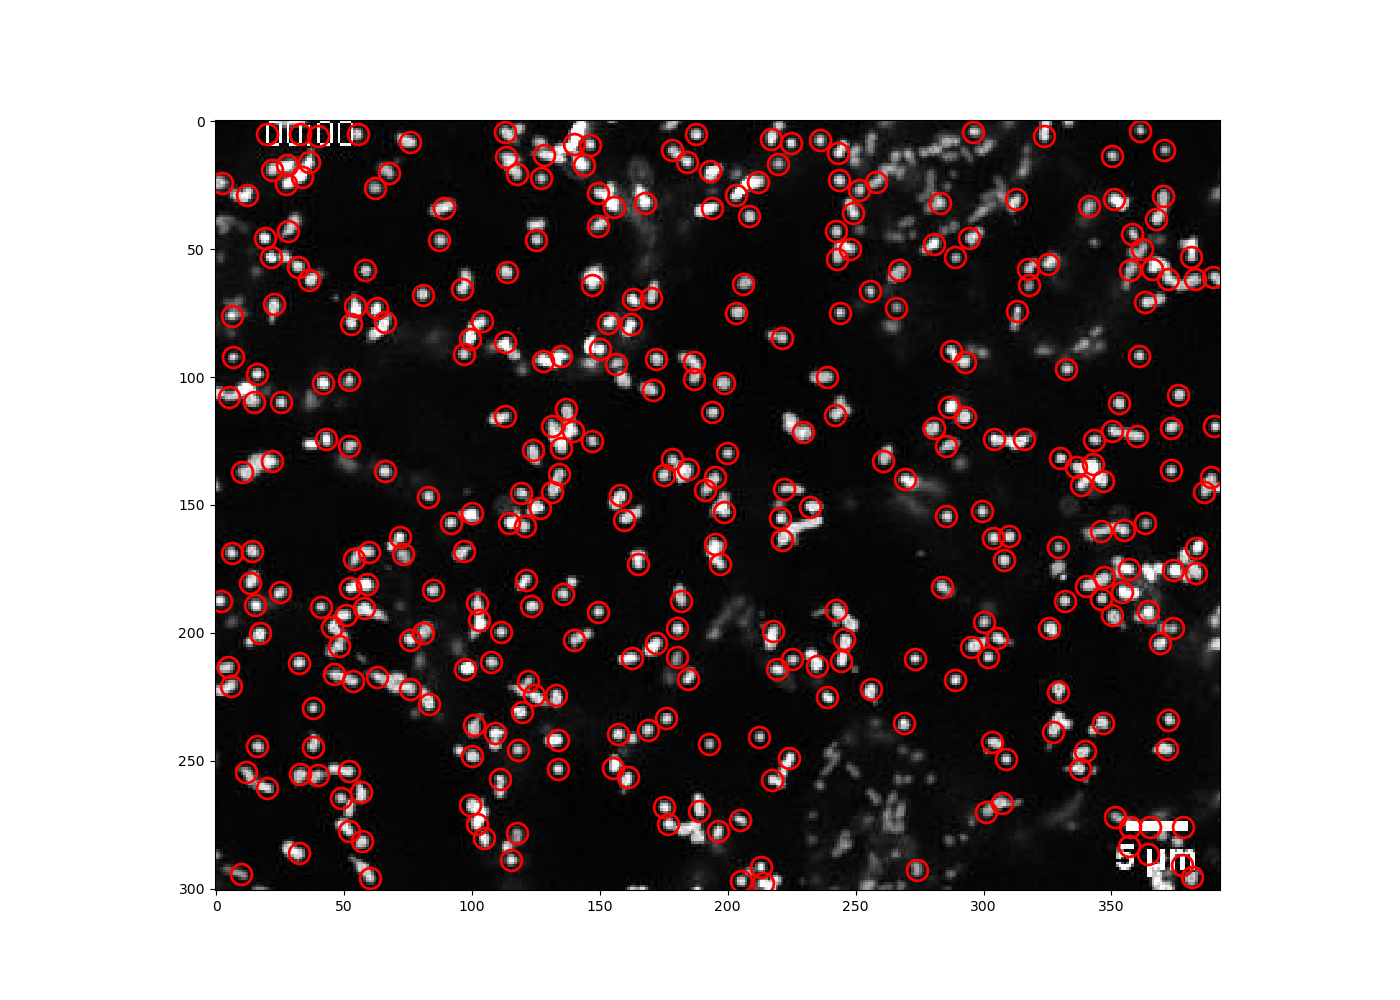
\includegraphics[scale=0.35]{Grafiken/trackpyBilder/locate_with_minmass_07(210).png}
    \caption{locate with 'mimass=210'}
    %\label{fig:bild_label}
\end{figure}


\begin{figure}[H]
    \centering
    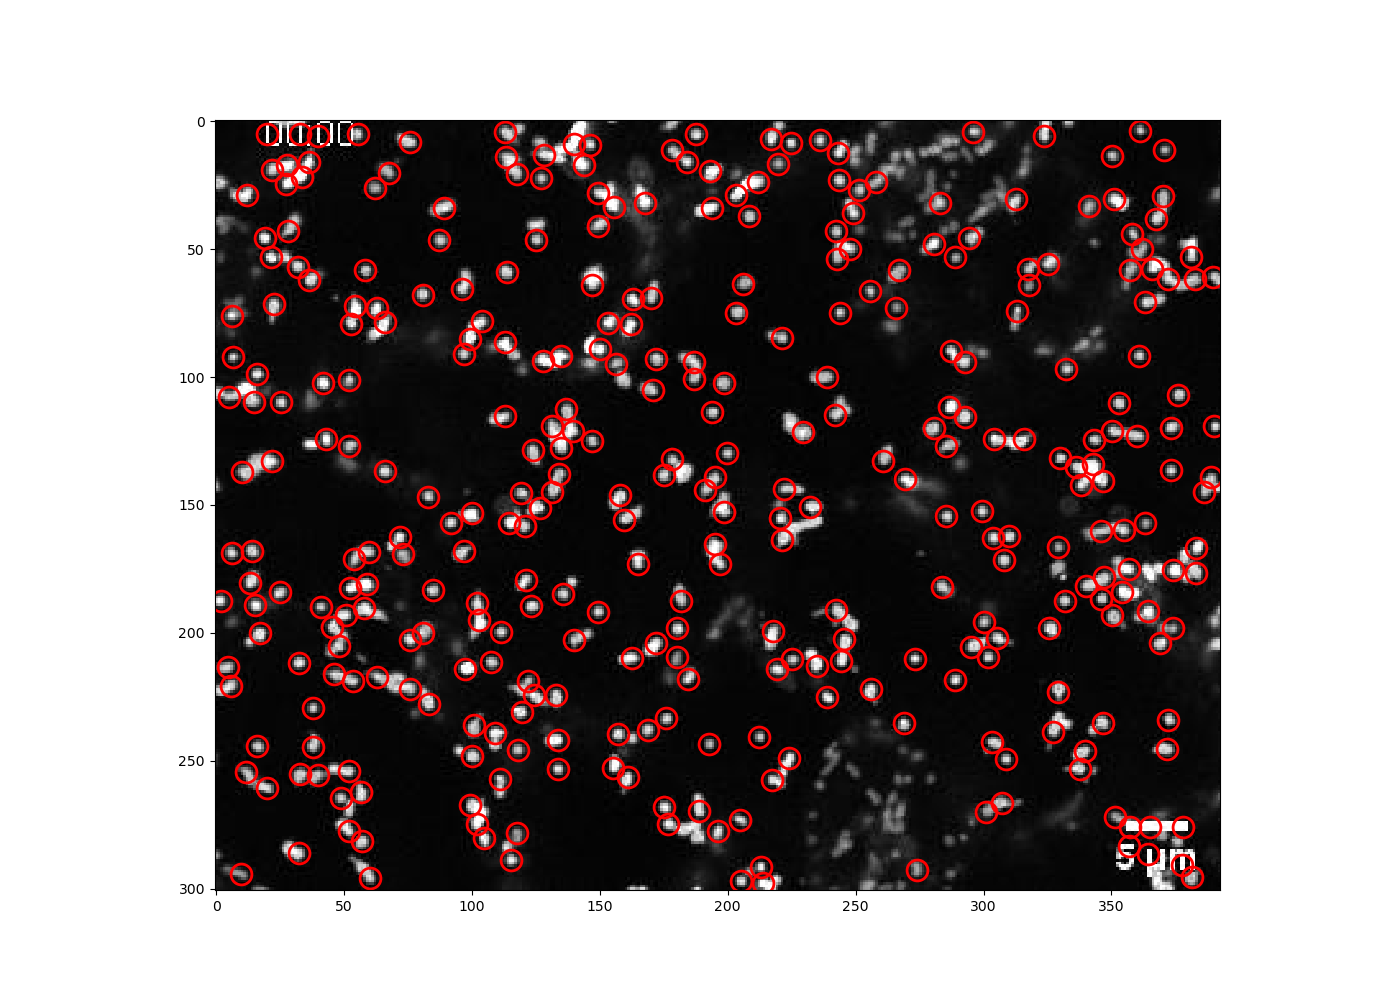
\includegraphics[scale=0.35]{Grafiken/trackpyBilder/locate_with_minmass_08(212).png}
    \caption{locate with 'mimass=212'}
    %\label{fig:bild_label}
\end{figure}


		\item {\Large \textbf{locate(f, d, minmass, sepration)}}: \\ \\
    			Hier wird es einfach Werte bei \texttt{separtion} ausprobiert, um auf die bessere Resultate zu kommen. 
    			Es wäre interessant zu erwähnen, dass es sich dabei um den minimalen Abstand zwischen zwei Teilchen handelt. Der Standardwert ist \textit{Durchmesser + 1}. In diesem Fall ist es 6. 
Mit diesem neuen Parameter werden wir versuchen, all jene Partikel zu eliminieren, die doppelt erkannt werden. Ohne die Qualität der bisherigen Erkennung zu beeinträchtigen.  

Denn es scheint offensichtlich, dass, wenn der Wert zu hoch ist, mehrere bisher erkannte Partikel nicht mehr erkannt werden. Weil sie zu nahe beieinander liegen.
Bei \texttt{separation = 6} bleibt die Erkennung unverändert und ergibt auch eine Anzahl von \textbf{345}.

\begin{figure}[H]
    \centering
    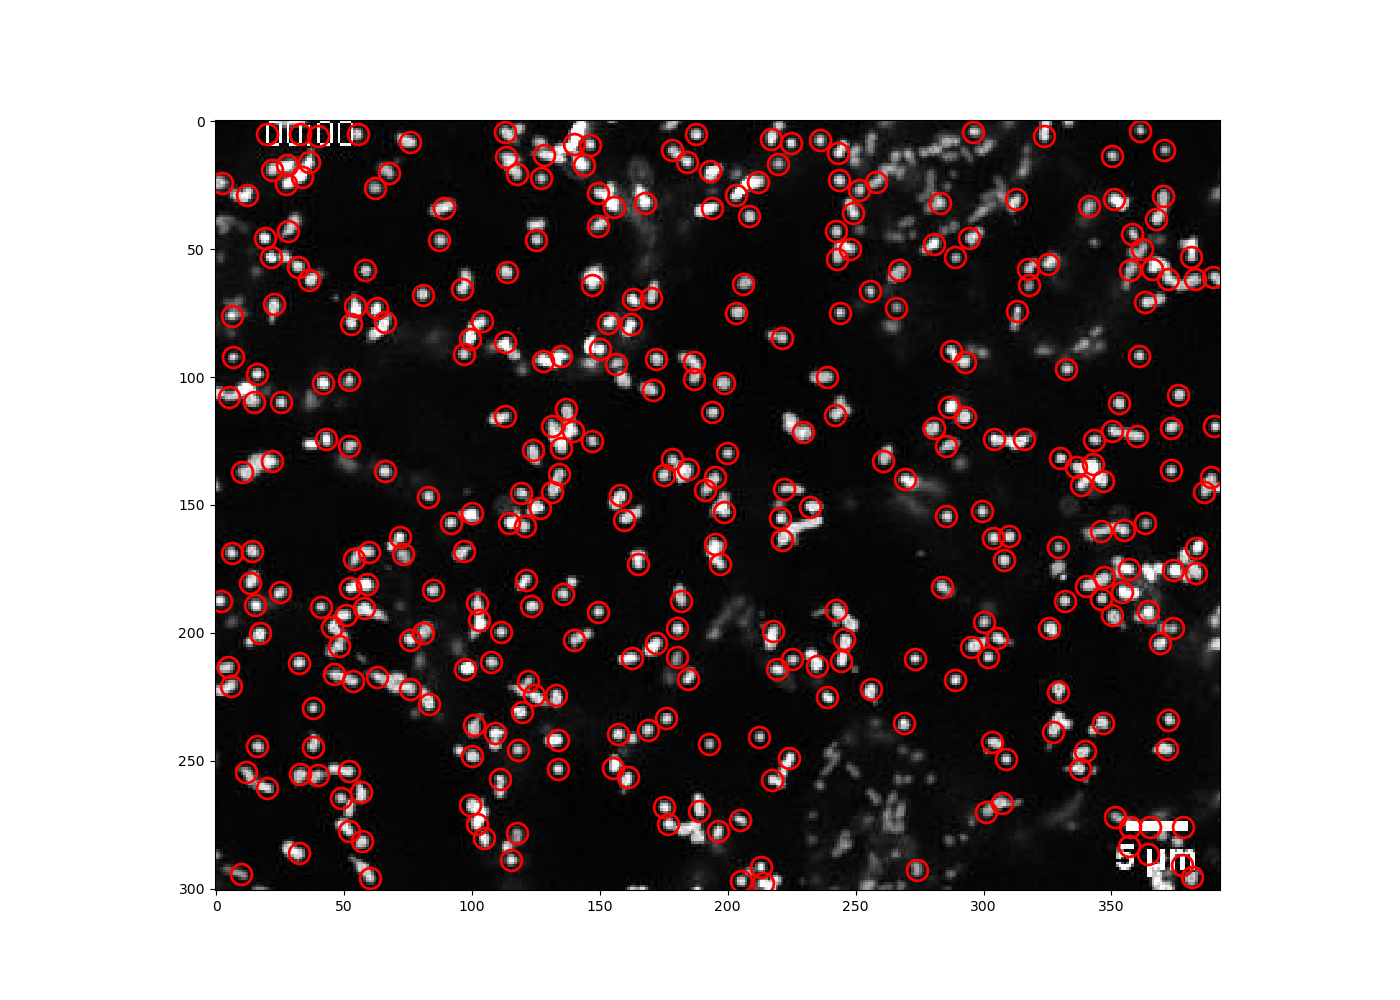
\includegraphics[scale=0.35]{Grafiken/trackpyBilder/locate_with_separation_(6).png}
    \caption{locate with 'sep=6.0'}
    %\label{fig:bild_label}
\end{figure}

Es wird dann als nächstes zuerst \textbf{7} als Parameterwert ausprobieren. Trotz der relativ kleinen Anzahl an insgesamt erkannten Partikel also \textbf{312}. Was auf dem folgenden Bild sichtbar ist, wird es ungefähr \textbf{10} gewünschte Partikel verloren. Diese sind in gelb auf dem Bild markiert. Natürlich hat der Parameterwert nicht nur Verschlechterung gezogen sondern auch positive Effekte. So ist es auch leicht in grün auf dem Bild Ausbesserungen zu sehen. Es handelt sich hier nämlich um \textbf{6} Partikel, die sich mehrfach erkennen lies. 
Allerdings, da die Anzahl an nicht mehr erkannte gewünschte Elemente größer ist als die von nicht gewünschten die eliminiert wurde, wird der Wert des Parameters dann nach unten korrigiert.
\begin{figure}[H]
    \centering
    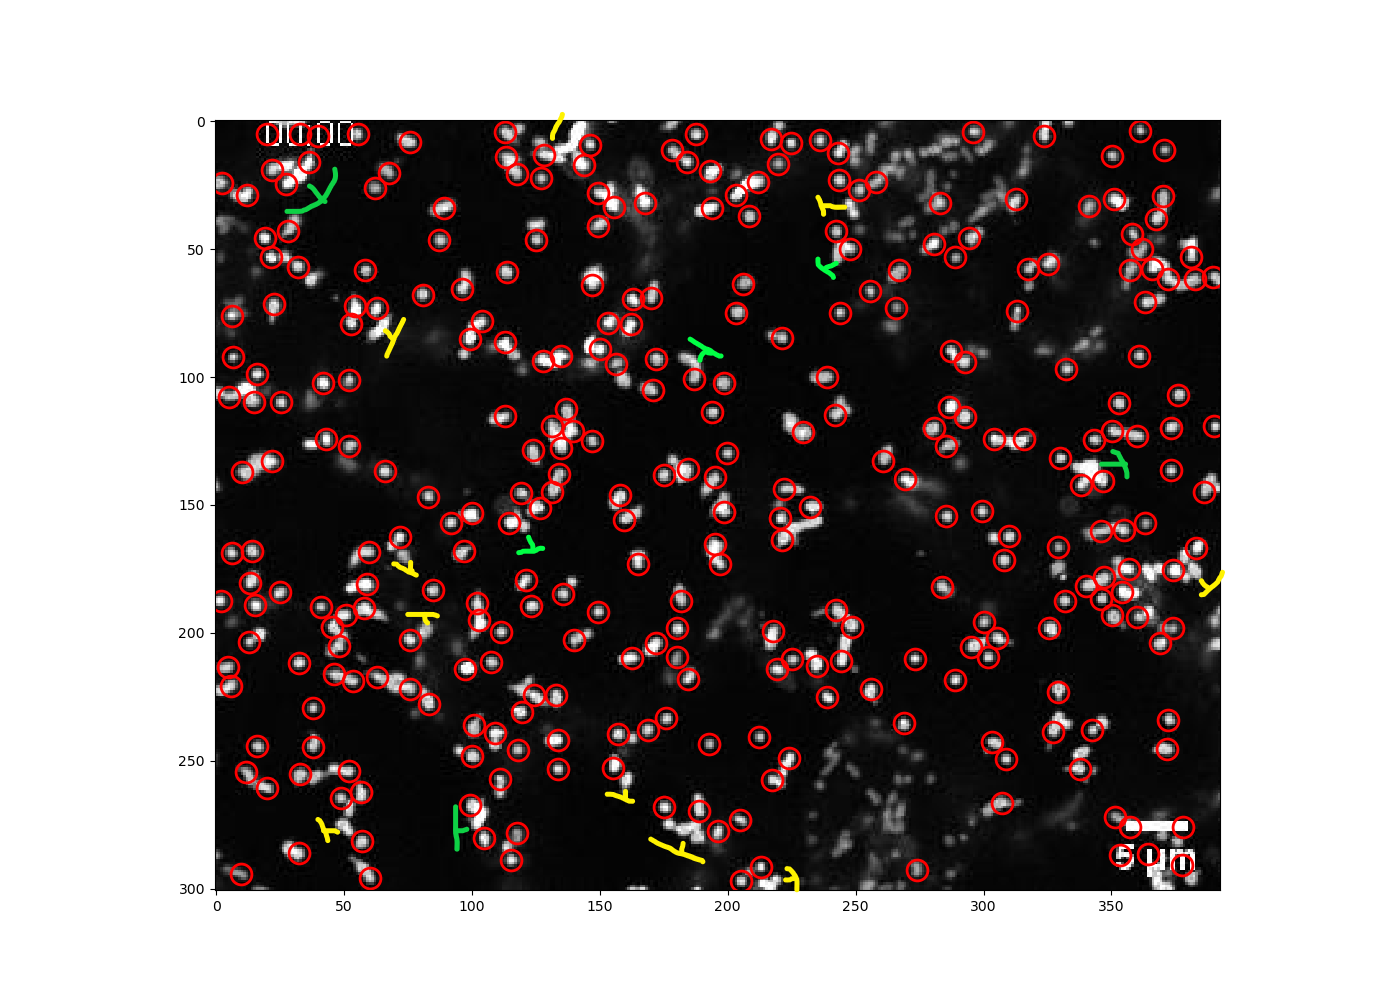
\includegraphics[scale=0.35]{Grafiken/trackpyBilder/locate_with_separation_(7).png}
    \caption{locate with 'sep=7.0'}
    %\label{fig:bild_label}
\end{figure}

Mit den aufeinanderfolgenden Werten \textbf{6.8, 6.7, 6.5 und 6.4} kommt es neben einigen Verbesserungen immer zu mehreren Verschlechterungen, die später mit anderen Parametern nur schwer zu korrigieren sind. 
Genau aus diesem Grund wird hier als  \textbf{separation} der Wert \textbf{6.3} betrachtet.
Wobei fast lediglich nur Verbesserungen zu notieren sind. 
\begin{figure}[H]
    \centering
    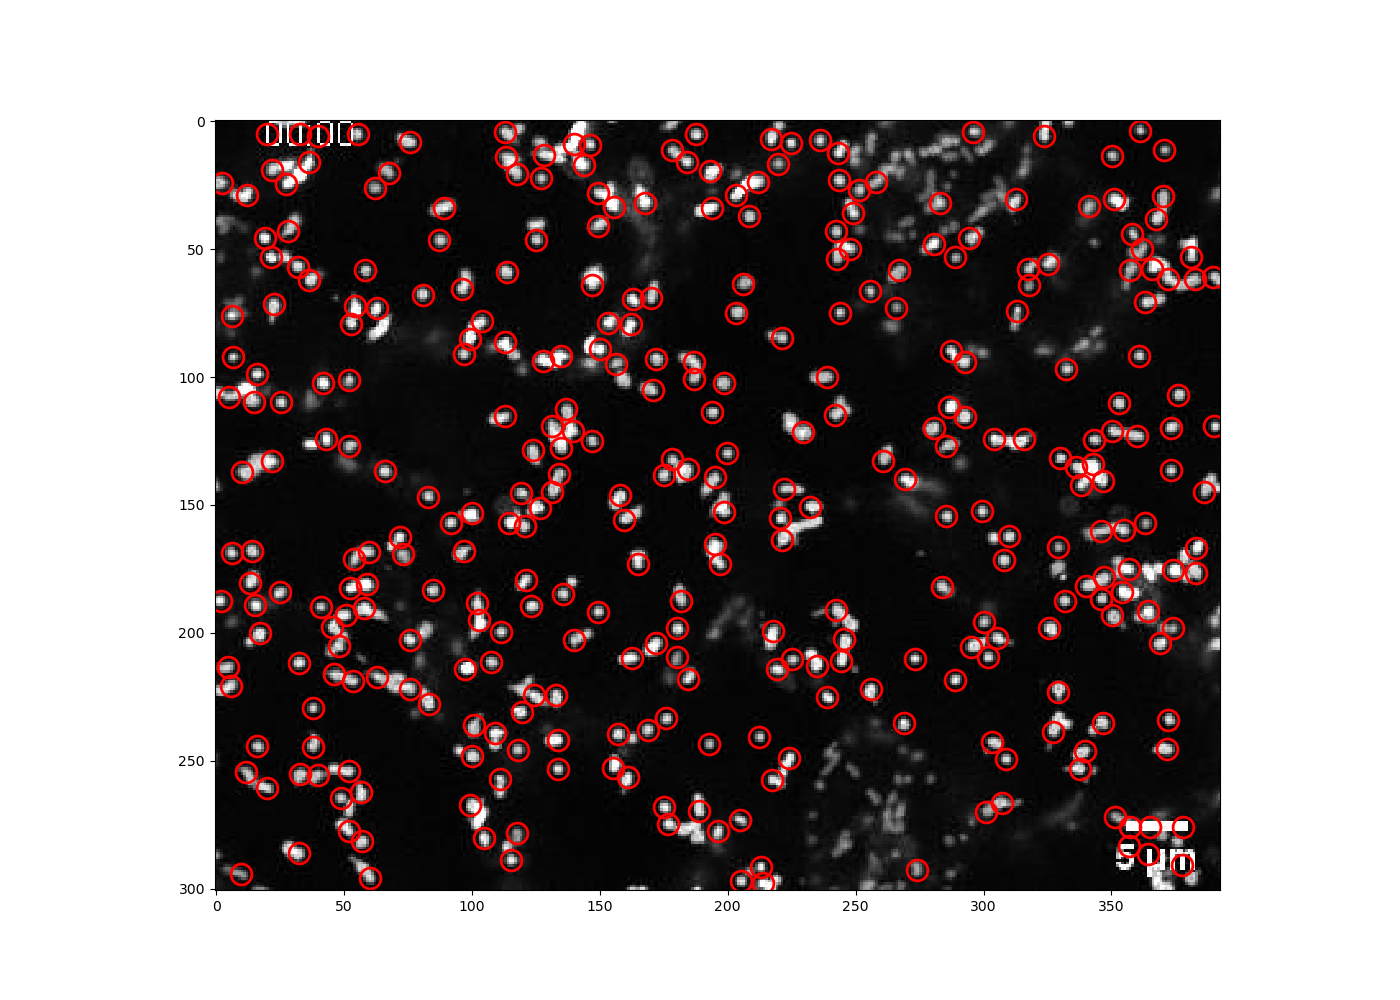
\includegraphics[scale=0.35]{Grafiken/trackpyBilder/locate_with_separation_(6,3).png}
    \caption{locate with 'sep=6.3'}
    %\label{fig:bild_label}
\end{figure}


%\item locate(frames[0], 11, minmass=1000.0, separation=2, noise\_size=1.5, topn=250):    \\ \\ 
%		Nachdem alle vorherige Parameter eingesetzt worden sind, wenn der Dataframe immer noch sanierungsbedürftig ist, wird auch \textit{topn} zum Einsatz gebracht. Dazu wird die Anzahl an bestehende unerwünschte Elemente geschätzt und von der gesamten Anzahl an gefundenen Elemente abgezogen. Somit wird \textit{topn} in dem Fall hier auf \textit{250} geschätzt. (siehe Bild)
%\begin{figure}[H]
%    \centering
%    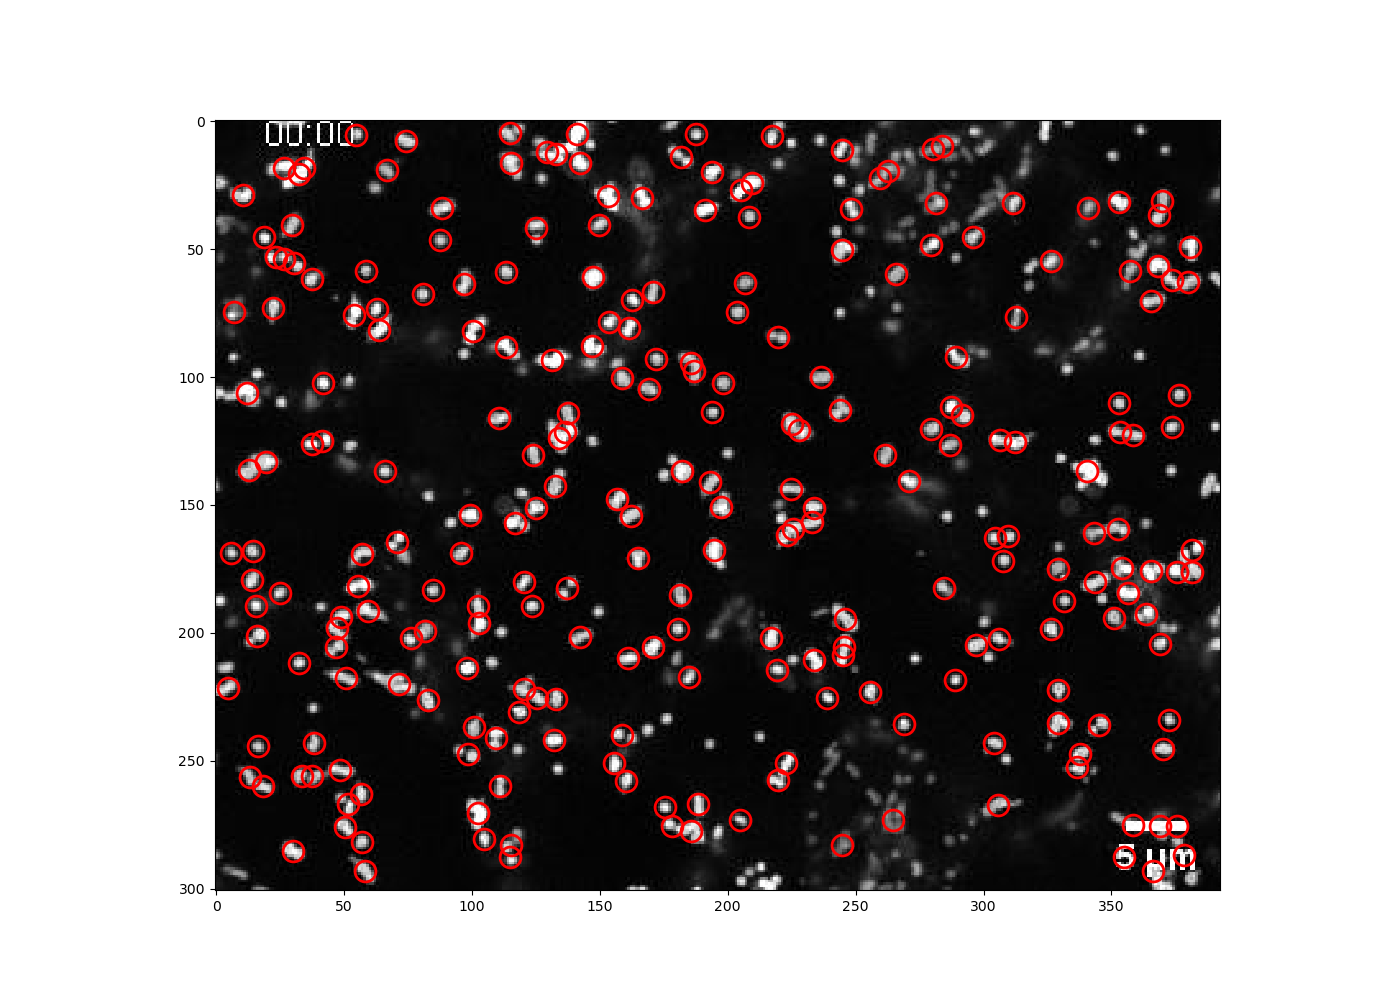
\includegraphics[scale=0.35]{Grafiken/trackpyBilder/locate_with_topn.png}
%    \caption{locate with 'topn=250'}
%    %\label{fig:bild_label}
%\end{figure}
\end{enumerate}
Es scheint hier wichtig zu erwähnen, dass es kein Parameter gibt, dessen Wert adäquat für alle Arten von Bildern oder Partikeln. So sollte es immer Parametrisierung als erster Schritt
durchgeführt werden.
Allerdings sind im konkreten Fall dieses Videos bzw. Bildes die Parameterwerte, die am besten geeignet erscheinen, wie folgt: \\
\begin{center}
{\Large \textit{locate(frames[0], 5, minmass=210, separation=6.3})}
\end{center}


\todo{kapitel1: Which  Library to use(avaible/)
Kapite2: Choosing good parameters for trackpy
kap3(Main Challenge):The Challenge of keeping particle count constant over frames.}


\subsection{Machine Learning}


